\documentclass[
%handout,
%draft,
compress]
{beamer}



\defbeamertemplate{section page}{mine}[1][]{%
  \begin{centering}
    {\usebeamerfont{section name}\usebeamercolor[fg]{section name}#1}
    \vskip1em\par
    \begin{beamercolorbox}[sep=12pt,center]{part title}
      \usebeamerfont{section title}\insertsection\par
    \end{beamercolorbox}
  \end{centering}
}
\setbeamertemplate{section page}[mine][]


\usetheme[authorwidth=.20,titlewidth=.50,datewidth=.30,section=true,subsection=true,]{Lund}
\setbeamertemplate{navigation symbols}{}
\usefonttheme[onlymath]{serif}
% automatic table of contents at every section
%\AtBeginSection[]{\frame{\tableofcontents[currentsection]}}
%\usepackage{pdfsync}
\usepackage[utf8x]{inputenc}
\usepackage{tikz}
\SetUnicodeOption{mathletters}
\usepackage{verbatim}
\hypersetup{ % information in the PDF file.
  pdftitle={Catch and throw\\Ball and Beam},%
  pdfauthor={Mattias Fält, Lucas Jimbergsson,\\Erik Nossborn, Iulia Stoica},
%  pdfsubject={Advanced Mathematics},
%  pdfkeywords={groups, triangles, algebras}
}

\usepackage{listings}

\title[Catch and Throw]{Catch and Throw\\Ball and Beam}
\author[]{Mattias Fält, Lucas Jimbergsson,\\Erik Nossborn, Iulia Stoica\\\vspace{1em}Supervisor -- Karl-Erik Årz\'{e}n}

%\date{2013-09-01}
\begin{document}
\frame{\titlepage}

\section*{Outline}

\frame
{
  \frametitle{Outline}
  \tableofcontents%[part=1]%,pausesections]%,shadesubsections]
}

\section{Introduction}
\frame{\sectionpage}
\begin{frame}
\frametitle{Problem Formulation}
\begin{itemize}
\item Dispatch a ball
\item Determine the weight
\item Choose the correct action:
\begin{itemize}
\item Small ball: Roll it into upper left cup
\item Medium ball: Throw into bucket
\item Large ball: Drop on the floor
\end{itemize}
\end{itemize}
\end{frame}


\begin{frame}
\frametitle{Difficulties}
\begin{itemize}
\item Controlling force on beam, not angle
\item Friction and bumps in beam
\item Temperature dependence
\end{itemize}
\end{frame}

\section{Overall Approach}
\frame{\sectionpage}
\begin{frame}
\frametitle{Initial Idea}
\begin{itemize}
\item Model the system
\item Find throw equations
\item Calculate trajectories
\item Stabilize with PID/LQG
\end{itemize}
\end{frame}

\begin{frame}
\frametitle{Initial Idea}

\begin{equation*}
\begin{pmatrix}
\dot{x}_{1}\\
\dot{x}_{2}\\
\dot{x}_{3}\\
\dot{x}_{4}
\end{pmatrix}=\begin{pmatrix}x_{2}\\
\frac{5}{7}\left(-g\sin(x_{3})+x_{1}x_{4}^{2}\right)\\
x_{4}\\
\frac{1}{J_B}(mgx_{1}\cos(x_3)+k_Bx_3+k_{u}u)
\end{pmatrix}
\end{equation*}
\begin{figure}
\centering
\scalebox{0.7}{\begin{tikzpicture}[scale=1.5]
\usetikzlibrary{patterns,snakes}
\definecolor{Darkgreen}{rgb}{0,0.4,0}
\tikzstyle{brace} = [decorate, decoration={brace, amplitude=5pt}]

\node[inner sep=0] (v0) at (0,0) {};
\node[inner sep=0] (v2) at (2,0.5) {};
\node[inner sep=0] (v1) at (-1,-0.25) {};

\draw[color=red]  (v1) edge (v2);

\node (v3) at (8,-2) {};
\node (v4) at (0,-2) {};
\node (v5) at (8,0) {};

\draw[ball color=blue] (2,0.6) circle (.1);

\draw[dashed,->] (v2) -- (4,1) node[pos=1,above] {$\dot{x}$};
\draw[dashed] (v0) -- (v5) {};
\draw[dashed] (v0) -- (v4) {};
\draw[brace] (v0) -- (v2) node[pos=0.5,above,yshift=6] {$l=x$};
\draw[brace] (v3) -- (v4) node[pos=0.5,below,yshift=-6] {$d_x$};
\draw[brace] (v5) -- (v3)  node[pos=0.5,right,xshift=5] {$d_y$};

 \draw[color=green] plot[smooth] coordinates {(v2) (4,0.6) (6,0) (8,-2)};
 
 
\node at (1.3,0.17) {$\phi$};

\path[clip] (2,0.5) -- (0,0) -- (2,0);
\node[circle,draw=Darkgreen, minimum size=90pt] at (0,0) (circ) {};

\end{tikzpicture}}
\end{figure}
\end{frame}

\begin{frame}
\frametitle{Initial Idea}
\[
\dot{x}=\left(d_{x}-l\cos(\phi)\right)\frac{\sqrt{g}}{\sqrt{2\cos(\phi)\left(d_{y}\cos(\phi)+d_{x}\sin(\phi)\right)}}.
\]
\begin{figure}
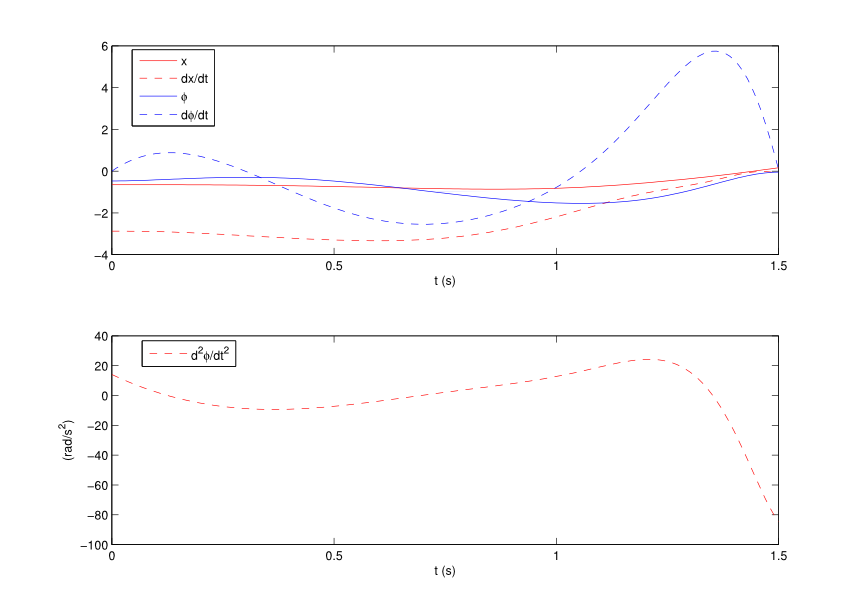
\includegraphics[width=0.7\textwidth]{ballbeammatlab}
\end{figure}

\end{frame}

\begin{frame}
\frametitle{Final Solution -- Heuristic Approach}
\begin{itemize}
\item Stabilize with cascaded PID
\item Use step/ramp references to move ball/beam
\item Throw using well times angle references
\end{itemize}
\end{frame}

\begin{frame}
\frametitle{Solutions to Difficulties}
\begin{itemize}
\item Controlling force on beam, not angle
\begin{itemize}
\item Use a lot of integral action in inner loop
\end{itemize}
\item Friction and bumps in beam
\begin{itemize}
\item Use a lot of integral action in outer loop
\end{itemize}
\item Temperature dependence
\begin{itemize}
\item Select robust and slow references
\end{itemize}
\end{itemize}
\end{frame}

\section{Controller Structure}
\frame{\sectionpage}
\begin{frame}
%\frametitle{}
\centering
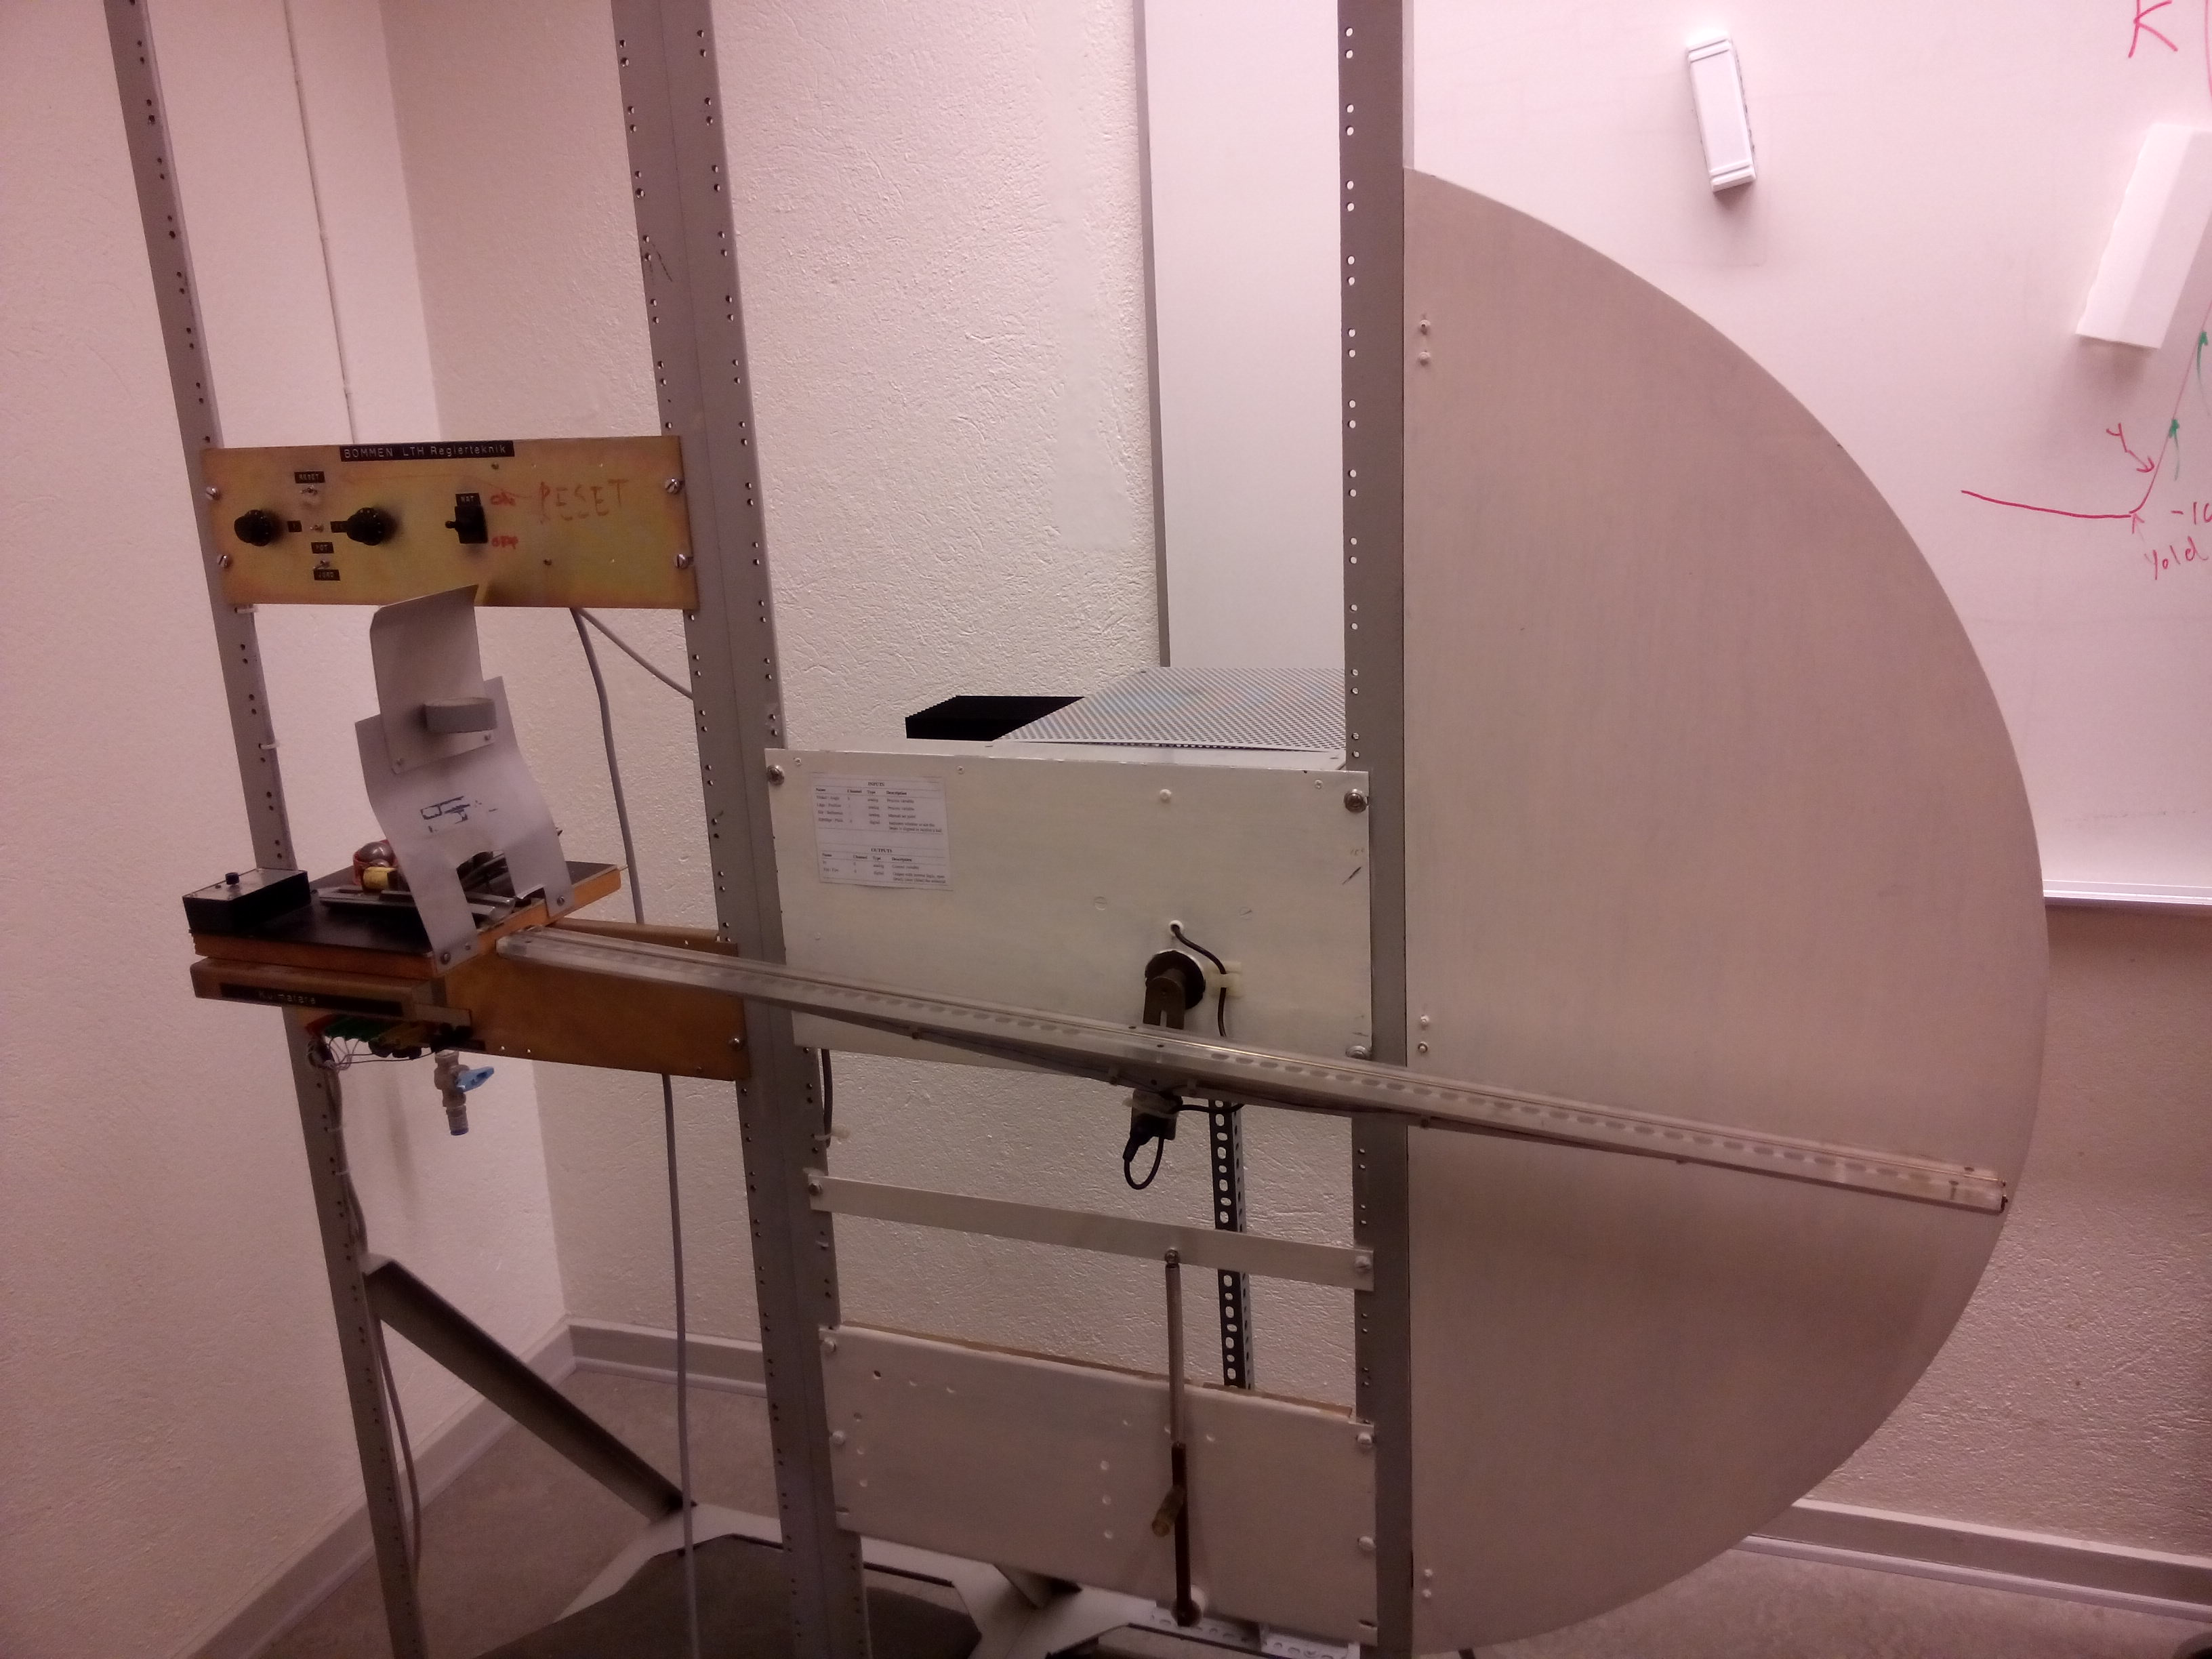
\includegraphics[width=0.8\textwidth]{figures/process_fig.jpg}
\end{frame}

\begin{frame}
\frametitle{Catch and Weigh Ball}
\centering
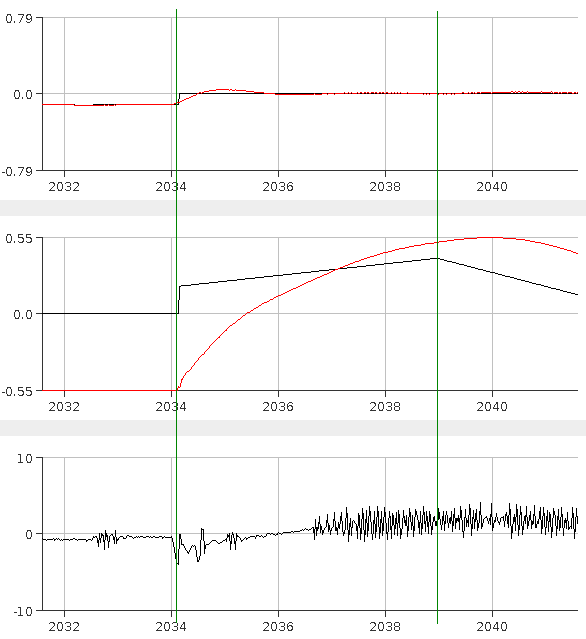
\includegraphics[height=0.83\textheight]{figures/weighmediumball-crop.png}
\end{frame}

\section{Program Structure}
\frame{\sectionpage}
\begin{frame}
\frametitle{Class Overview}
\centering
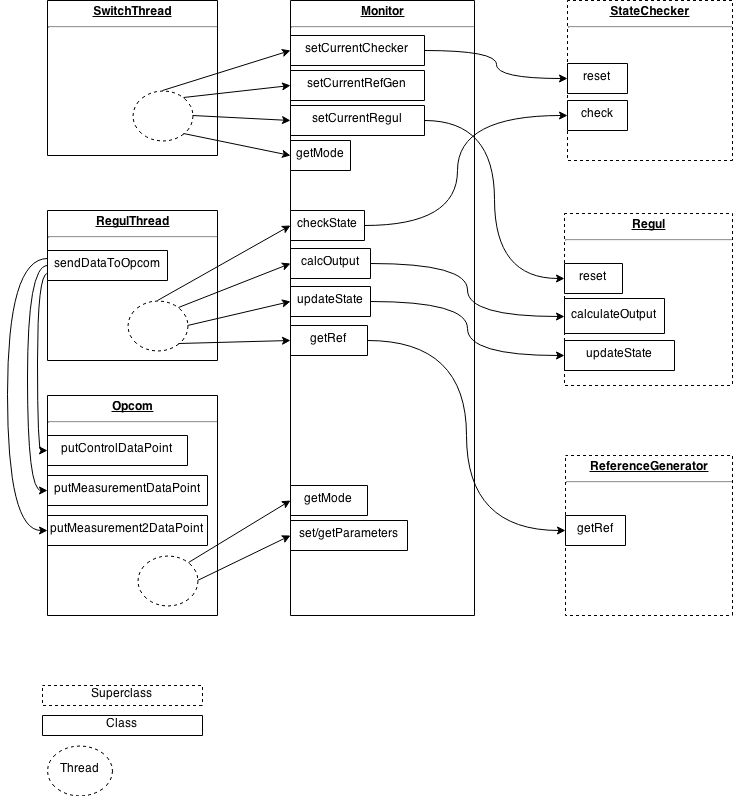
\includegraphics[height=0.83\textheight]{figures/UML.png}
\end{frame}

\begin{frame}[fragile]
\frametitle{RegulThread}
\begin{lstlisting}[language=java,xleftmargin=3em]
periodic loop {
    getInputs();
    calcOutput();
    setOutput();
    updateState();
    checkState();
}
\end{lstlisting}
\end{frame}

\begin{frame}[fragile]
\frametitle{SwitchThread}
\begin{lstlisting}[language=java,xleftmargin=3em]
...
synchronized (mon) {
    mon.setBallRegul();
    mon.setRefGenRamp(startPos,weighPos);
}
//calls wait():
mon.setConstBallCheck(weighPos,tolerance); 
switch(checkWeight()){
...
\end{lstlisting}
\end{frame}

\section{Results and Conclusions}
\frame{\sectionpage}
\begin{frame}
\frametitle{Step Responses}
\centering
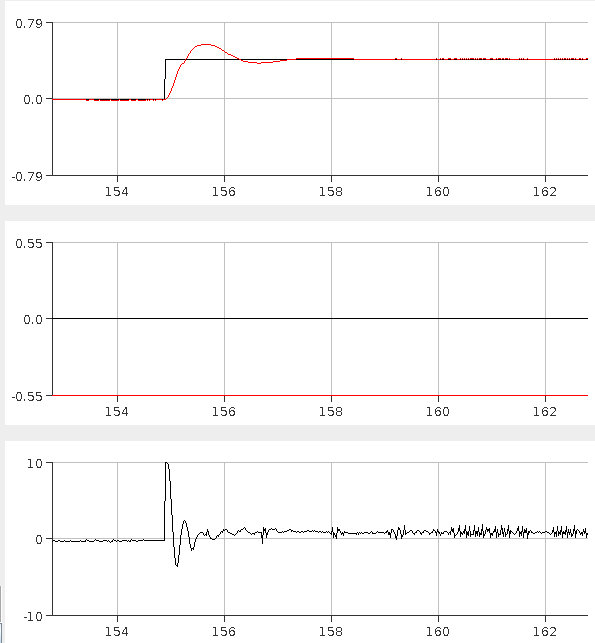
\includegraphics[width=0.45\textwidth]{figures/stepresponsebeam-crop.png}
\hspace{1em}
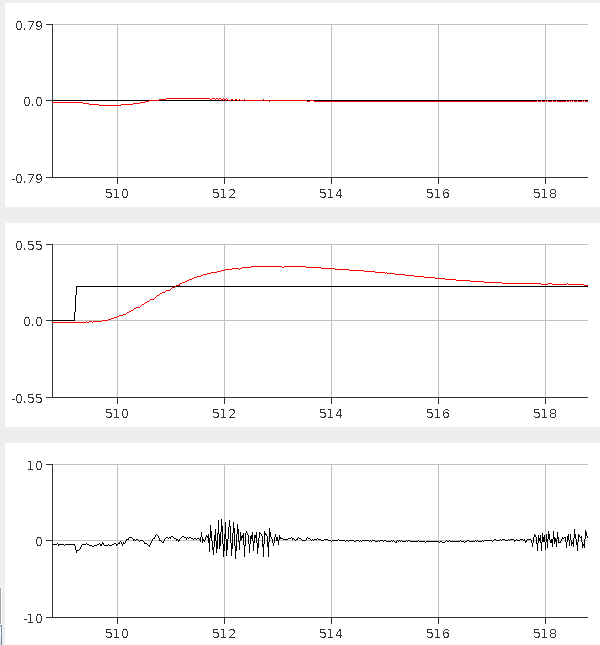
\includegraphics[width=0.45\textwidth]{figures/stepresponseball1-crop.png}
\end{frame}

\begin{frame}
\frametitle{Catching and Weighing}
\centering
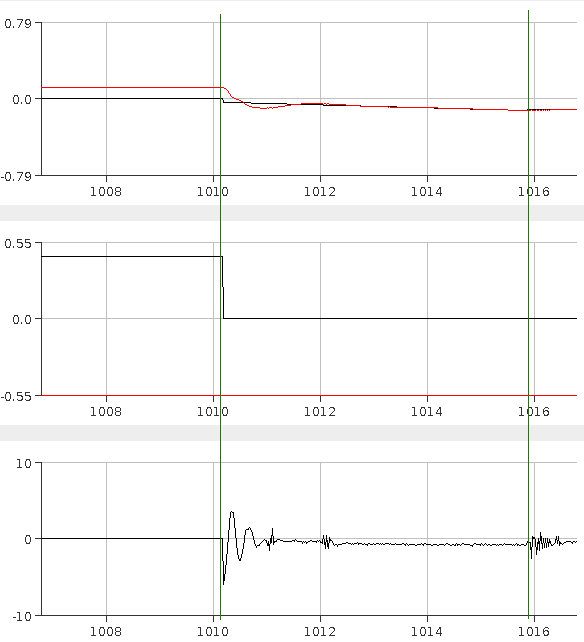
\includegraphics[width=0.45\textwidth]{figures/topickupposition-crop.png}
\hspace{1em}
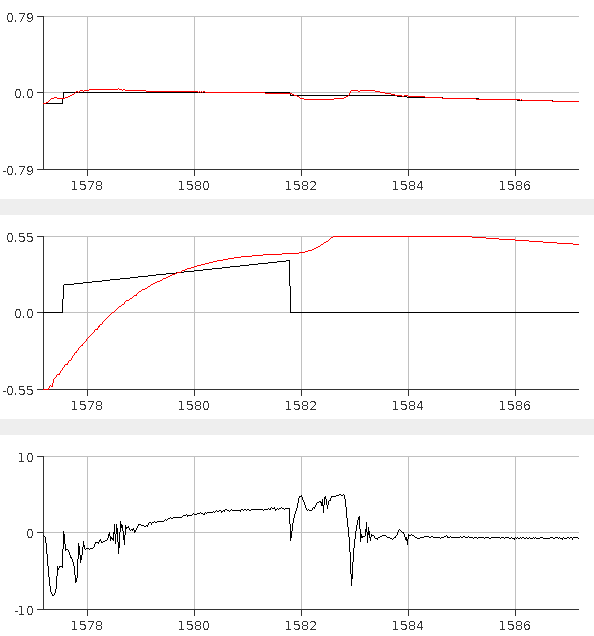
\includegraphics[width=0.45\textwidth]{figures/weighanddroplargeball-crop.png}
\end{frame}

\begin{frame}
\frametitle{Small and Medium Balls}
\centering
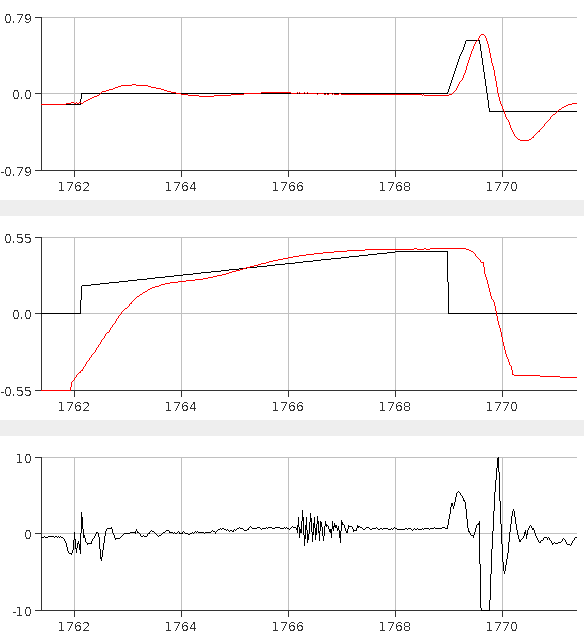
\includegraphics[width=0.45\textwidth]{figures/weighandthrowsmallball-crop.png}
\hspace{1em}
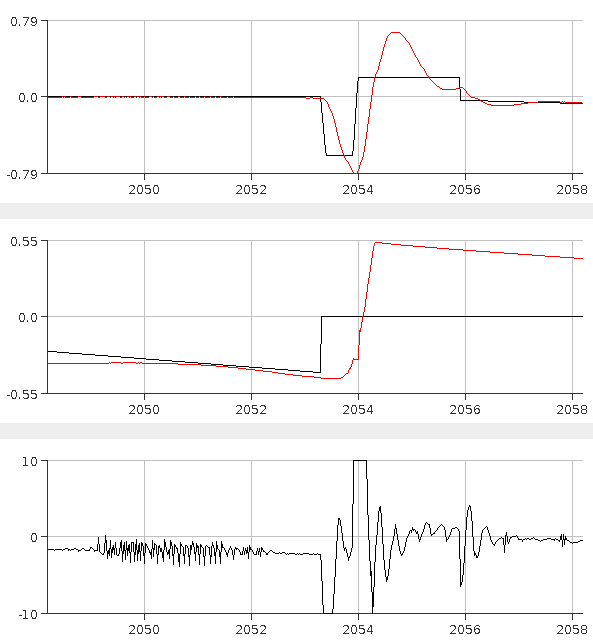
\includegraphics[width=0.45\textwidth]{figures/throwmediumball-crop.png}
\end{frame}

\begin{frame}
\frametitle{Numerical Optimization Approach}
\centering
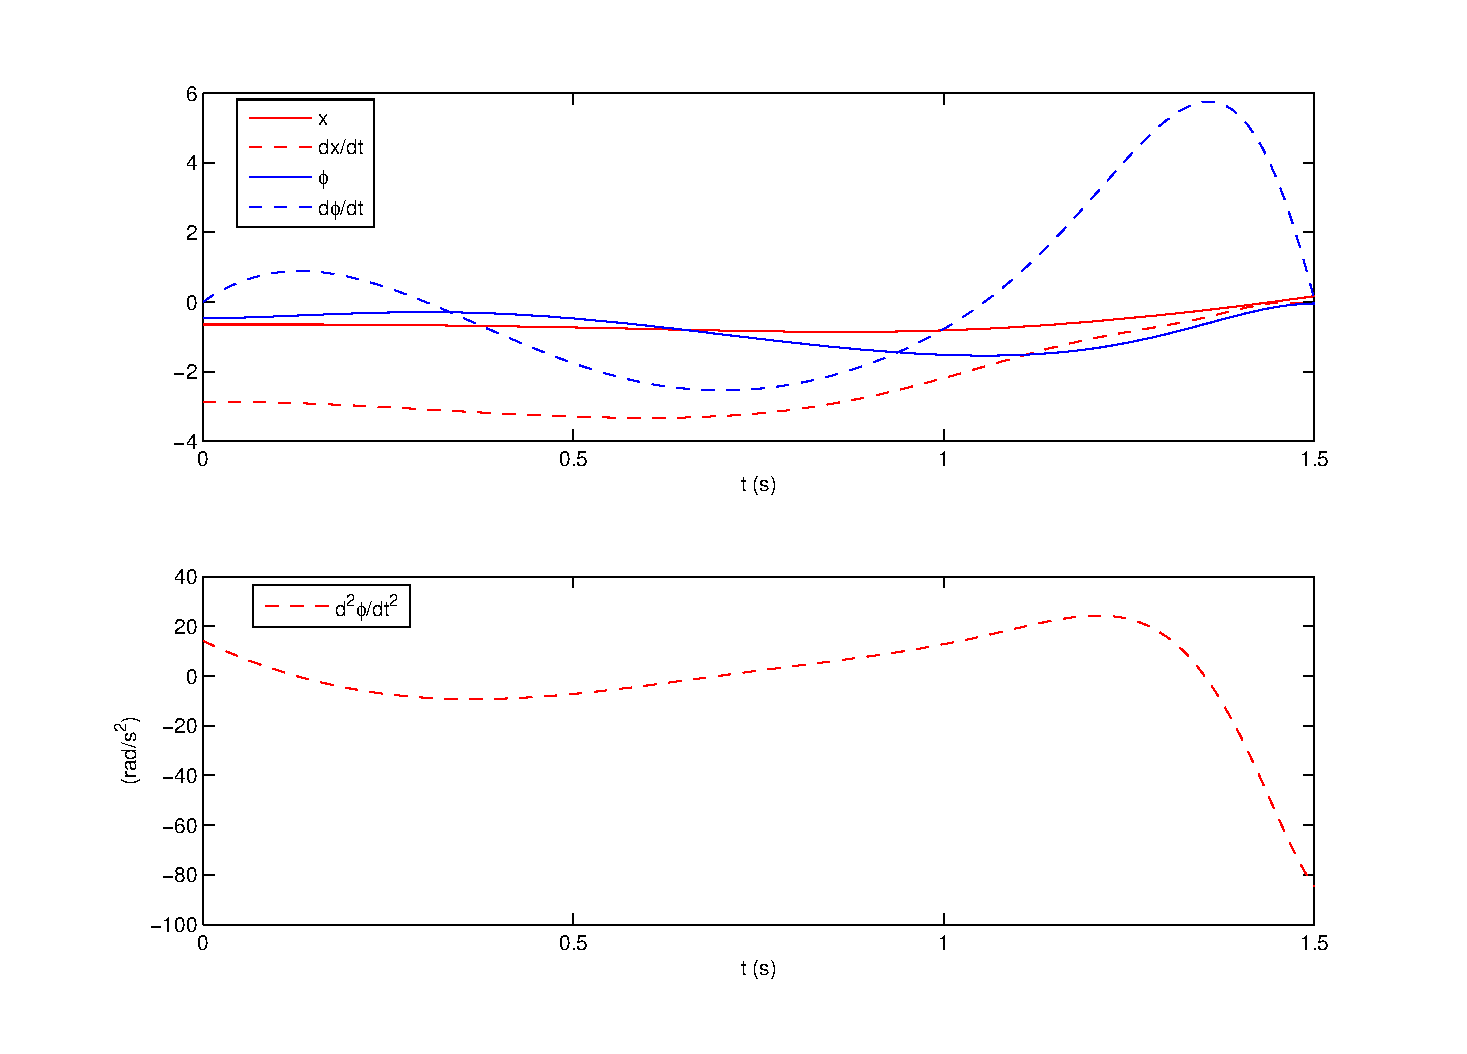
\includegraphics[width=0.9\textwidth]{ballbeammatlab.eps}
\end{frame}

\end{document}

